\documentclass{article}
\usepackage[utf8]{inputenc}
\usepackage{graphicx}
\usepackage{subfigure}
\usepackage{listings}
\usepackage{color} %red, green, blue, yellow, cyan, magenta, black, white
\definecolor{mygreen}{RGB}{28,172,0} % color values Red, Green, Blue
\definecolor{mylilas}{RGB}{170,55,241}
\usepackage{amsmath}

\title{ASSIGNMENT 2 NEURAL NETWORKS: BOOSTING}
\author{Álvaro González, Ismael Peruga}
\date{February 2017}


\begin{document}

\maketitle
\section{Introduction}
In this assignment, a boosting algorighm has to be implemented in order to classify pictures between faces and non-faces, specifically the AdaBoost algorithm, which was explained in lesson number 4. The basic concept of this algorithm is to train different weak classifier sequentially where the next weak classifier tries to correct the errors from the previous classifier (this is done by using different weights for each sample and giving higher or lower values for the samples wrongly classified and correctly classified respectively).

To train the different classifiers, a large number of pictures are given where some of them correspond to faces and the rest to non-faces. The input for the algorithm is the Haar-features for each image, these features are just filters applied to the images and they measure the contrast from different positions in the image (the number of Haar-features needed to train the classifier is up to us and is a task to find the best number).

\section{Data}
To perform this assignment, a set of images including faces and non-faces is used. A subset of these kind of images is seen in figure \ref{fig:facesExample}.

\begin{figure}[htbp]
\centering
\subfigure{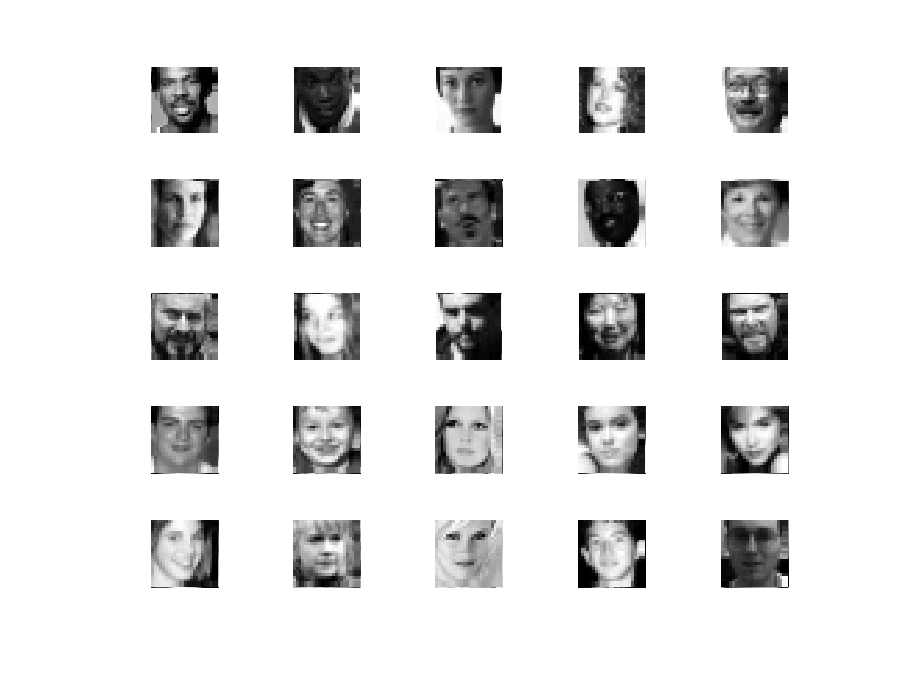
\includegraphics[width=100mm]{images/facesExample}}
\subfigure{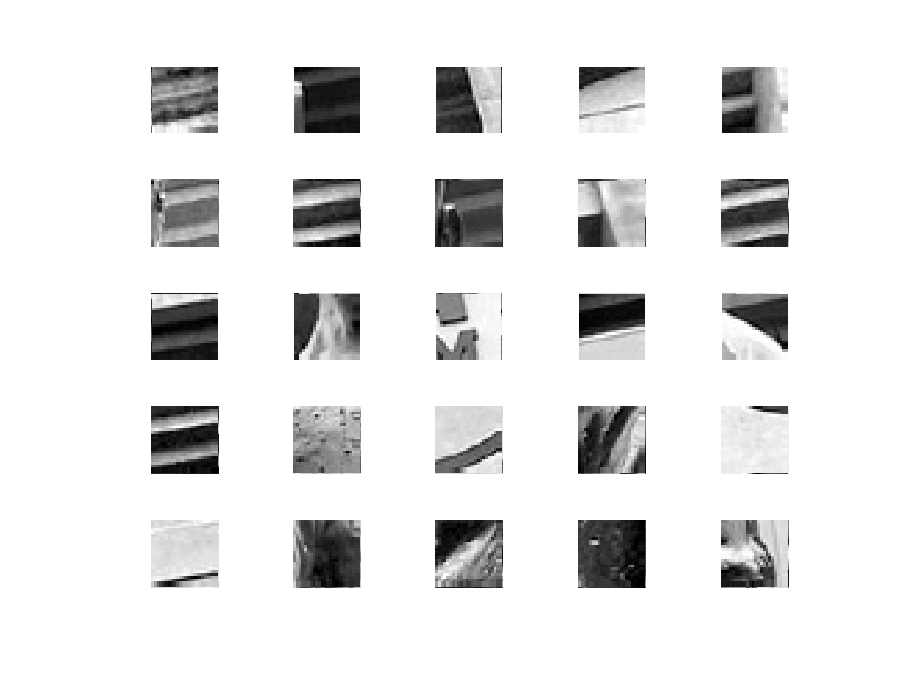
\includegraphics[width=100mm]{images/non-facesExample}}
\caption{Examples of faces and non-faces images} \label{fig:facesExample}
\end{figure}

\section{Implementation}
To implement Adaboost, we have proceeded like it was explained at lesson number 4. What we have done is a function that implemented training of the classifiers. As inputs we set the number of weak classifiers, the input samples (Haar-features of the test data) and the desired label of each image. As outputs we get the polarity, the threshold, the features and the weight $\alpha$ of each classifier. 

For each classifier we look for the threshold that minimizes the weighted error. To do so, all the features of the input data are used as threshold and the one that has the minimum error is selected to be the threshold of a weak classifier. Then $\alpha$ for the classifier is calculated and the weights of the samples are updated taking in account if the sample has been correctly classified or not. We do this until we have set the threshold and the feature for all classifiers. At the end, the strong classifier is calculated as the wheighted sum of each weak classifier. 

\section{Results}

\subsection{Performance factors}

To measure how good is the implementation, we are going to see how it behaves with the training data varying the number of Haar-features and the number of weak classifiers. 

In figure \ref{fig:accuracyOnTrainingFeaturesClassifiers} it can be seen how the accuracy in the training data varies depending on the number of Haar-features and on the number of weak classifiers. (This have been done using 200 training images, 100 of each class).

\begin{figure}[h]
\centering
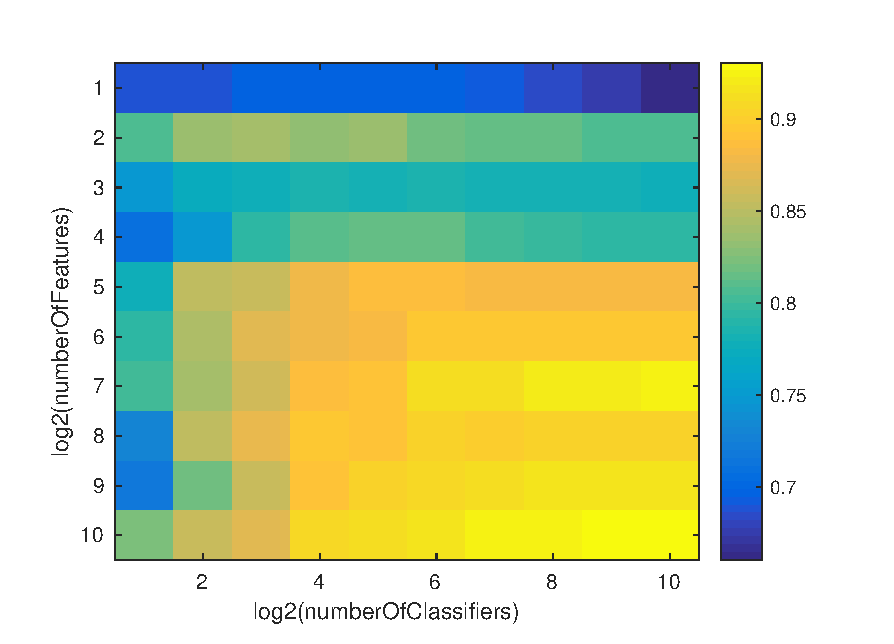
\includegraphics[height=4cm]{images/accuracyOnTrainingFeaturesClassifiers}
\caption{Accuracy on training data depending on the number of weak classifiers}
\label{fig:accuracyOnTrainingFeaturesClassifiers}
\end{figure}

This is the matrix that represents the figure \ref{fig:accuracyOnTrainingFeaturesClassifiers} 

$$\begin{pmatrix}
0,689 & 0,689 & 0,693 & 0,695 & 0,694 & 0,696 0,691 & 0,683 & 0,674 & 0,660 \\ 
0,804 & 0,836 & 0,837 & 0,831 & 0,834 & 0,820 0,816 & 0,815 & 0,807 & 0,804 \\ 
0,745 & 0,771 & 0,777 & 0,786 & 0,779 & 0,783 0,779 & 0,779 & 0,778 & 0,778 \\
0,707 & 0,746 & 0,793 & 0,808 & 0,814 & 0,813 0,803 & 0,798 & 0,795 & 0,793 \\
0,777 & 0,850 & 0,856 & 0,879 & 0,885 & 0,885 0,882 & 0,880 & 0,881 & 0,881 \\
0,795 & 0,844 & 0,870 & 0,879 & 0,881 & 0,893 0,892 & 0,895 & 0,896 & 0,894 \\
0,801 & 0,841 & 0,860 & 0,886 & 0,891 & 0,912 0,913 & 0,918 & 0,920 & 0,922 \\
0,731 & 0,851 & 0,875 & 0,895 & 0,891 & 0,901 0,899 & 0,904 & 0,903 & 0,903 \\
0,717 & 0,817 & 0,858 & 0,890 & 0,903 & 0,908 0,909 & 0,916 & 0,916 & 0,916 \\
0,823 & 0,857 & 0,871 & 0,908 & 0,912 & 0,916 0,925 & 0,926 & 0,928 & 0,930 \\
\end{pmatrix}$$


This is the matrix of the accuraccy depending on the number of weak classifier and Haar-features. Each row is the base 2 logarithm of the number of Haar-features and the columns are the base 2 logarithm of the number of weak classifiers. It can be seen that once the number of features is 32 and the number of weak classifiers is 16, the accuracy starts getting close to 0.9 on the training data. Of course, the more features and the more weak classifiers are used, the best performance is obtained, but it saturates.

Using 200 images to train (100 faces and 100 non-faces) and letting fixed the number of Haar-features also in 100, the results for the accuracy on test data depending on the number of weak classifier is plotted in figure  \ref{fig:accuracyOnTestDONumClassifiers}

\begin{figure}[h]
\centering
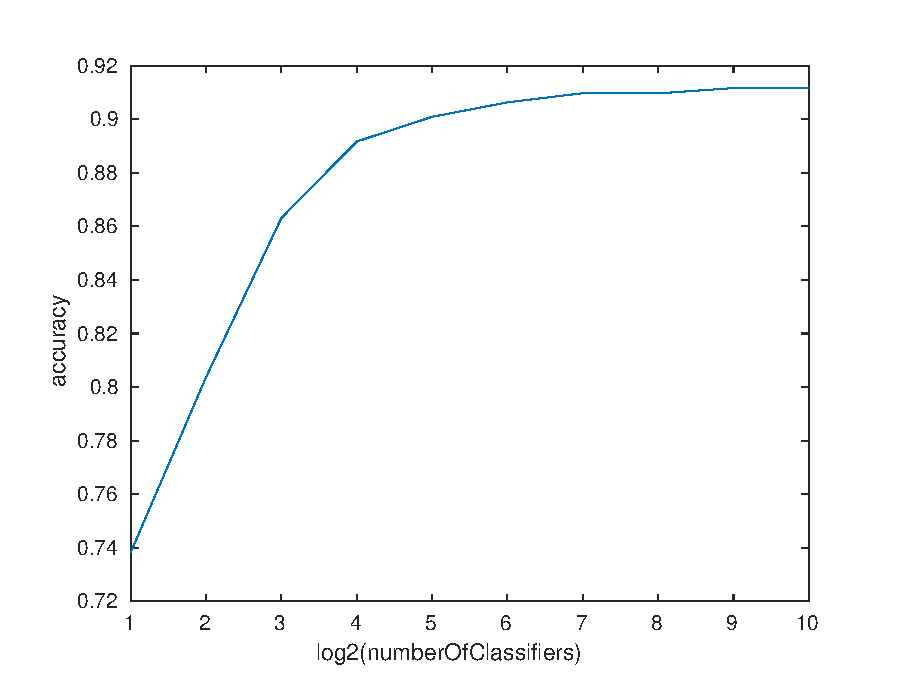
\includegraphics[height=6cm]{images/accuracyOnTestDONumClassifiers}
\caption{Accuracy on testing data depending on the number of weak classifiers}
\label{fig:accuracyOnTestDONumClassifiers}
\end{figure}

When the number of classifiers is above 32, the accuracy on the test data is good enough (above 0.9) and maybe the overhead of training more classifiers (which implies more computational power and time) is not necessary since the behaviour is better than the required. It happens something similar with the number of Haar-features used.

Since the requirements say that the accuracy should be tested over at least the half of the available data, this is the result using a total of 12388 images (faces + non-faces). The number of weak classifiers trained is 64 and the number of Haar-features is 32. The accuracy obtained is 0.8585. If the number of features is 64 and the number of classifiers is 128, the accuracy then improves to 0.9099.

One last try is to use 400 images for training, the number of features of 256 and 512 weak classifiers. The number of test data images is 11988. The accuracy is 0.9339, which is an improvement from before.

%podemos poner una tabla con estos valores

\subsection{Examples of misclassified images}

In figures \ref{fig:hard_faces} and \ref{fig:hard_nonfaces} we show some examples of faces misclassified as non-faces or reversed.

\begin{figure}[h]
\centering
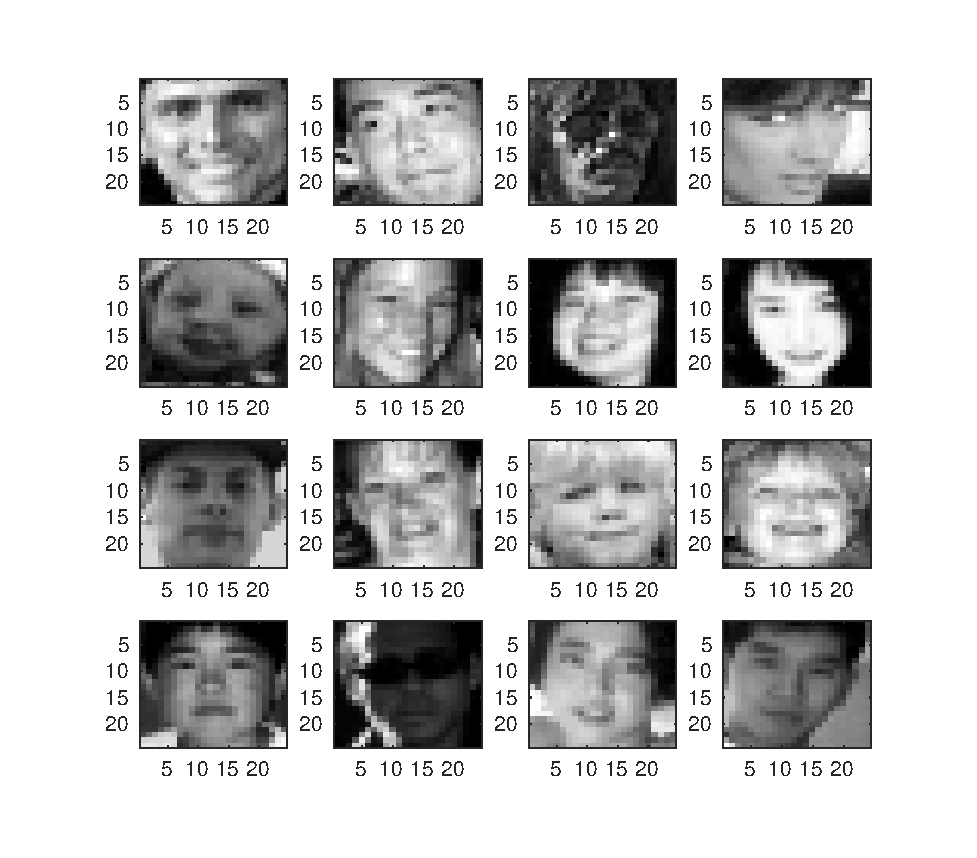
\includegraphics[height=6cm]{images/hard_faces}
\caption{Examples of misclassified faces as non-faces images.}
\label{fig:hard_faces}
\end{figure}

\begin{figure}[h]
\centering
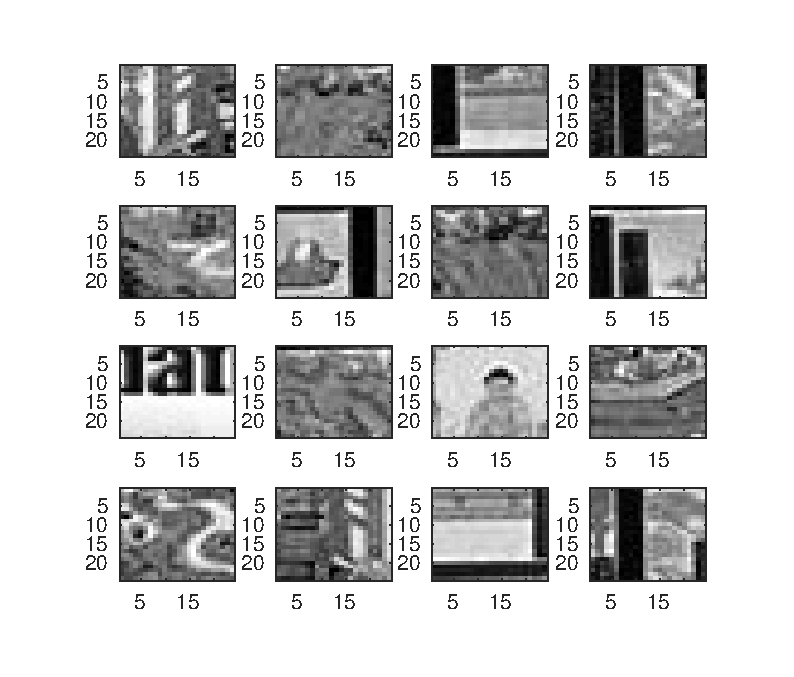
\includegraphics[height=6cm]{images/hard_nonfaces}
\caption{Examples of misclassified non-faces as faces images.}
\label{fig:hard_nonfaces}
\end{figure}

\begin{figure}[h]
\centering
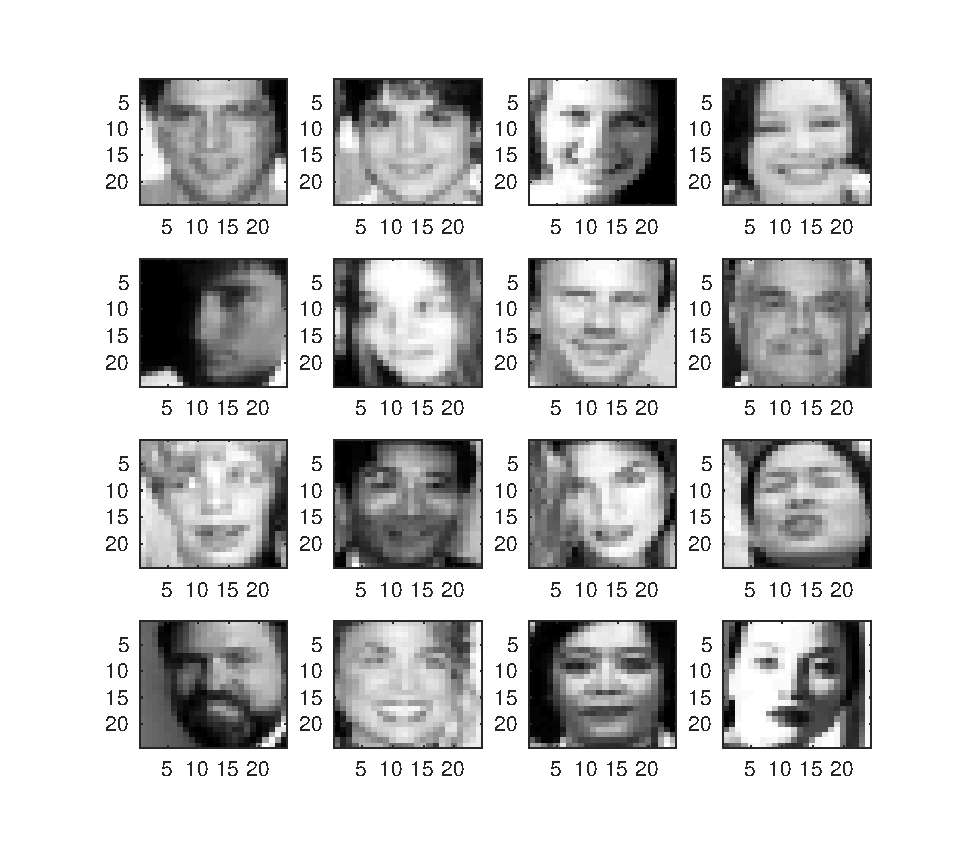
\includegraphics[height=6cm]{images/easy_faces}
\caption{Examples of correctly classified faces.}
\label{fig:easy_faces}
\end{figure}

Just as a curiosity, we calculated the mean of all faces (figure \ref{fig:mean_all}), the mean of correctly classified faces (figure \ref{fig:mean_correct}), and the mean of missclassified faces (figure \ref{fig:mean_miss}). We see that the mean of correctly classified faces is almost indistingible to the mean of all faces, but the mean of misclassified faces is notably different (but still a recognizable face).

\begin{figure}[h]
\centering
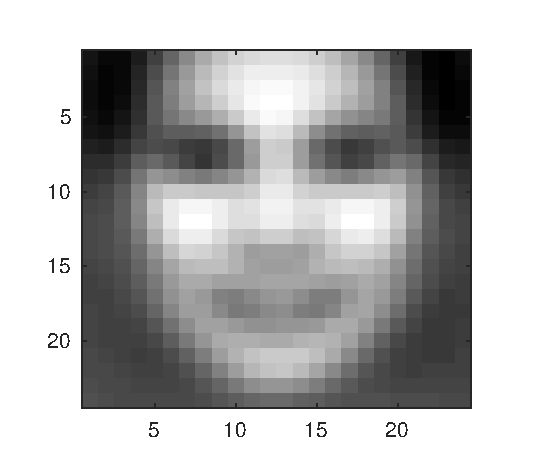
\includegraphics[height=3cm]{images/mean_all}
\caption{Mean-face of all faces.}
\label{fig:mean_all}
\end{figure}

\begin{figure}[h]
\centering
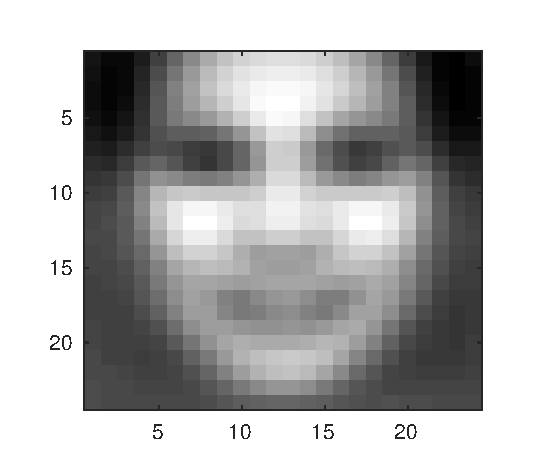
\includegraphics[height=3cm]{images/mean_easy}
\caption{Mean-face of correctly classified faces.}
\label{fig:mean_correct}
\end{figure}

\begin{figure}[h]
\centering
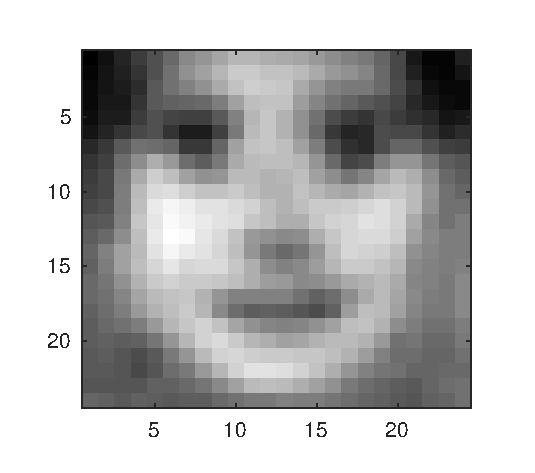
\includegraphics[height=3cm]{images/mean_hard}
\caption{Mean-face of missclassified faces.}
\label{fig:mean_miss}
\end{figure}

\section{Discussion and conclusion}

We think that we obtained good results with a very simple algorithm and a low amount of features/classifiers. It is also important to consider that the Haar features are obtained randomly and they still allow us to obtain more than 90\% of accuracy in unseen data. We could expect better results with less but more hand-designed Harr features. 

However, this algorithm is quite simple and the results will be far from perfect. This is mainly because the obtained model only weightd simple features, and is sensitive to outliers and noise. It can be useful for simple and fast applications. For the more complex ones, maybe it can be used as a meta-algorithm with other less weak classifiers.


\end{document}
